\chapter{State of the Art}\label{cap:estadoDeLaCuestion}

In this chapter, we will explore the fundamental concepts and classical techniques on which our chess engine is based. This includes game trees and search algorithms. Each section will provide an overview of the concepts and tools used by our engine, and additionally we will explain the workflow we followed to get better versions of our engine.

\section{Game trees}

Sequential games, such as chess or tic-tac-toe, where players take turns alternately, unlike simultaneous games, can be represented in a game tree or graph. In this representation, the root node corresponds to the initial position from which we search for the best move, and each subsequent node represents a possible option or game state, forming a tree-like structure. The tree has a height or depth, which refers to the number of turns alternating between black and white from the root node to the leaf nodes.

\begin{figure}[H]
    \centering
    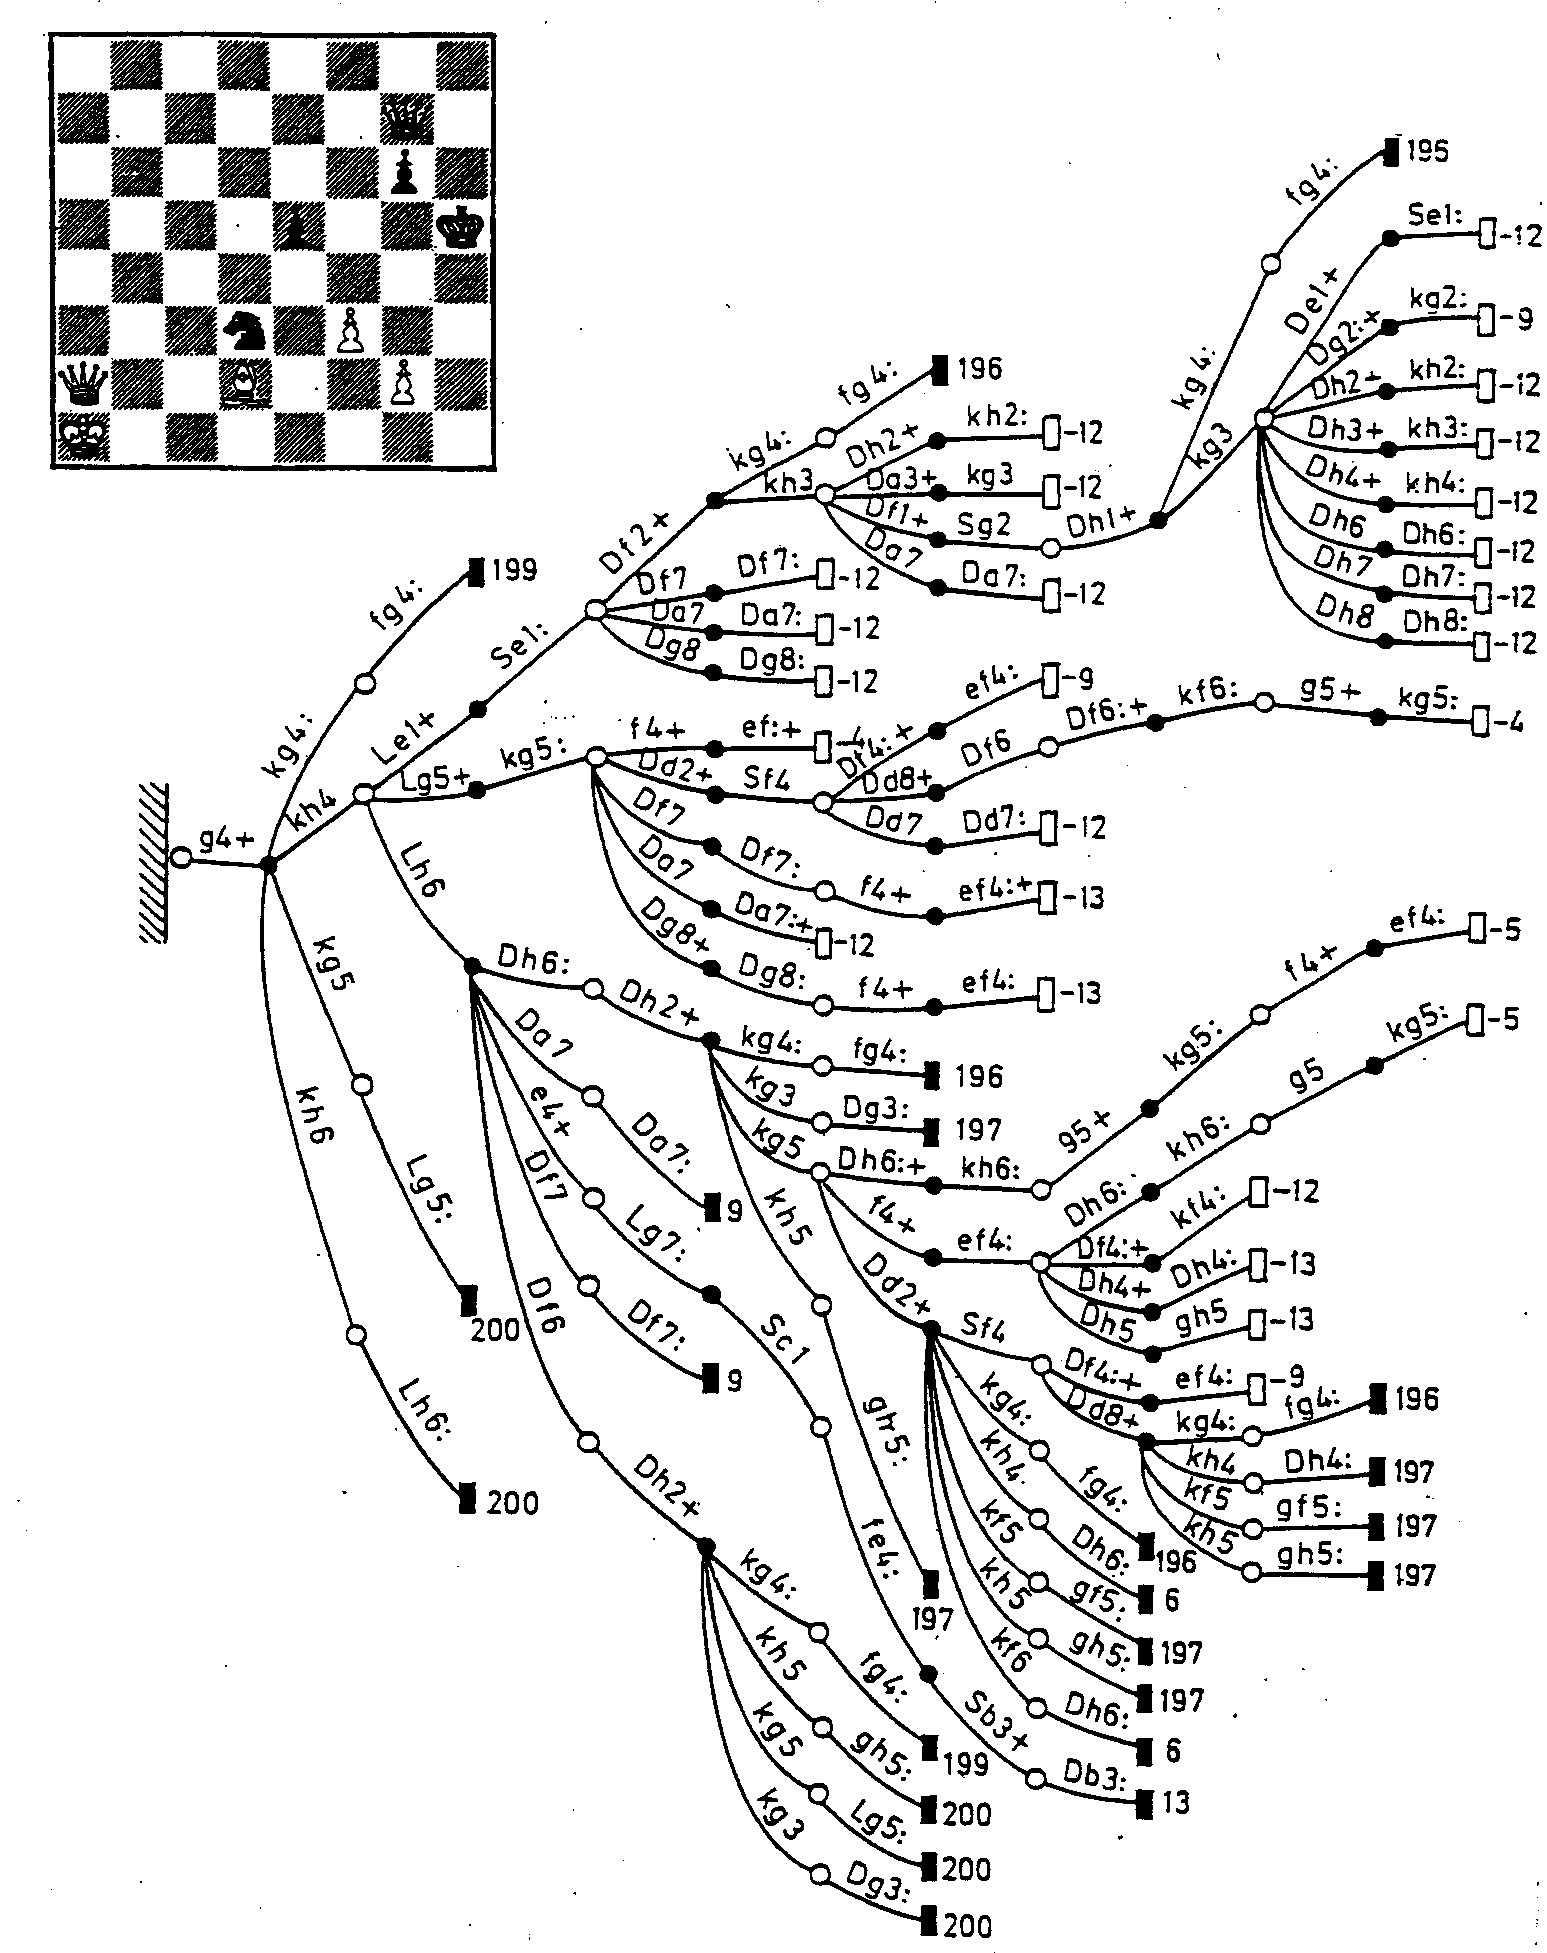
\includegraphics[width=0.35\textwidth]{Imagenes/chess-game-tree.jpg}
    \caption{Illustration of a game tree for a chess position~\cite{BotvinnikLongRangePlanning}.}\label{fig:game-tree}
\end{figure}

\noindent The depth of a chess game tree is important because it determines the extent to which it will be analysed and evaluated. A depth of 1 represents all possible moves for the current player or side to move, while a depth of 2 includes the opponent's responses to those moves. As the depth increases, the tree grows exponentially, making it computationally expensive to explore all possible states.

\vspace{1em}

\noindent In~\cref{fig:game-tree}, the shaded cluster of lines on the left represents the part of the game tree corresponding to previous moves leading up to the current position. From there, only a subset of possible continuations is drawn, illustrating the immense complexity of chess. Claude Shannon estimated that the number of possible chess games is around $10^{120}$, a value known as the \textit{Shannon number}~\cite{Shannon1950}. This astronomical figure makes it computationally infeasible to represent or analyze the entire game tree, motivating the use of search algorithms and pruning techniques to explore only the most relevant branches, which are explained in the following section.

\section{Search algorithms}

There are different approaches to analyze and find the best move from a position. Some of these search algorithms are: Depth-First Search (DFS), Best-First Search (not to be confused with Breadth-First Search or BFS but they are related), and Parallel Search.

\vspace{1em}

\noindent Note that these search algorithms are the foundation of more advanced and practical algorithms used today. That's why explaining them is essential to understand the underlying principles.

\paragraph{Depth-First Search} refers to the process of exploring each branch of a tree or graph to its deepest level before backtracking. Unfortunately, in chess, this cannot be possible as mentioned in the last section. This is because the number of possible moves grows exponentially with the depth of the search tree, leading to the so-called combinatorial explosion. To address this, depth-first search is often combined with techniques like alpha-beta pruning to reduce the number of nodes evaluated, making the search more efficient while still exploring the tree deeply.~\cref{lst:dfs} illustrates the working of the DFS algorithm.

\vspace{1em}

\begin{lstlisting}[caption={Pseudocode of the Depth-First Search algorithm.}, label={lst:dfs}, frame=single, numbers=left, xleftmargin=15pt]
Procedure DFS(Graph G, Node v):
    Mark v as visited
    For each neighbor w of v in G.adjacentEdges(v):
        If w is not visited:
            Recursively call DFS(G, w)
\end{lstlisting}

\noindent DFS visits nodes by marking them as visited (line 2) and recursively explores all adjacent nodes until no unvisited nodes remain (lines 3 to 5). It has a worst-case performance of $O(|V| + |E|)$ and worst-case space complexity of $O(|V|)$, with $|V| = \text{number of nodes}$ and $|E| = \text{number of edges}$.

\vspace{1em}

\noindent In practice, especially in chess, a bounded or depth-limited version of DFS is often used. In bounded DFS, the search is restricted to a maximum depth, preventing the algorithm from exploring the entire tree. This approach allows the algorithm to focus on the most relevant positions.

\paragraph{Best-First Search} refers to the way of exploring the most promising nodes first. It is similar to a breadth-first search but prioritizes some nodes before others. They typically require significant memory resources, as they must store a search space (the collection of all potential solutions in search algorithms) that grows exponentially.

\vspace{1em}

\begin{lstlisting}[caption={Pseudocode of the Best-First Search algorithm.}, frame=single, numbers=left, xleftmargin=10pt, breaklines=true]
Procedure BestFirstSearch(Graph G, Node start, Node goal):
    Create an empty priority queue PQ
    Add start to PQ with priority 0
    Mark start as visited

    While PQ is not empty:
        Node current = PQ.pop()
        If current is the goal:
            Return the path to the goal

        For each neighbor w of current in G.adjacentEdges(current):
            If w is not visited:
                Calculate priority for w (e.g., using a heuristic)
                Add w to PQ with the calculated priority
                Mark w as visited
\end{lstlisting}

\noindent In this case, the priority queue contains nodes along with their associated priorities, which are determined by a heuristic function. This process is commonly referred to as branch and bound, where the algorithm explores branches of the search tree according to their heuristic value.

\paragraph{Parallel Search} refers to mulithreaded search, a technique used to accelerate search processes by leveraging multiple processors.

\vspace{1em}

\noindent Next, we will discuss one of the most widely used search algorithms in chess engines: the minimax algorithm.

\subsection{Minimax algorithm}\label{sec:minimax}

The \textbf{minimax} algorithm is a decision making algorithm that follows Depth-First Search (DFS) principles. It is based on the assumption that both players play optimally, with one player (the maximizer) trying to maximize his score and the other player (the minimizer) trying to minimize his score. It explores the game tree to evaluate all possible moves and determines the best move for the current player.~\cref{lst:minimax} has the pseudocode of the algorithm:

\vspace{1em}

\begin{lstlisting}[caption={Pseudocode of the Minimax algorithm.}, label={lst:minimax}, frame=single, numbers=left, xleftmargin=15pt, breaklines=true]
Procedure Minimax(Node position, Integer depth, Boolean maximizingPlayer):
    If depth == 0 or position is a terminal node:
        Return the evaluation of the position

    If maximizingPlayer:
        Integer maxEval = -Infinity
        For each child of position:
            Integer eval = Minimax(child, depth - 1, False)
            maxEval = max(maxEval, eval)
        Return maxEval
    Else: // minimizingPlayer
        Integer minEval = +Infinity
        For each child of position:
            Integer eval = Minimax(child, depth - 1, True)
            minEval = min(minEval, eval)
        Return minEval
\end{lstlisting}

\begin{figure}[H]
    \centering
    \begin{tikzpicture}[
        level distance=1.5cm,
        level 1/.style={sibling distance=4cm},
        level 2/.style={sibling distance=2cm},
        circleNode/.style={circle, draw, minimum size=1cm, inner sep=0pt},
        squareNode/.style={rectangle, draw, minimum size=1cm, inner sep=0pt}
    ]
        % Root node
        \node[squareNode] (root) {3}
            child {node[circleNode] (b) {3}
                child {node[squareNode] (d) {3}}
                child {node[squareNode] (e) {5}}
            }
            child {node[circleNode] (c) {2}
                child {node[squareNode] (f) {2}}
                child {node[squareNode] (g) {9}}
            };

        \node[left=1.2cm] at (root) {MAX};
        \node[left=1.2cm] at (b) {MIN};
        \node[left=1.2cm] at (d) {MAX};

        % Edges
        \draw[-{Stealth}, draw=red] (b) -- (root);
        \draw[-] (root) -- (c);
        \draw[-{Stealth}, draw=red] (d) -- (b);
        \draw[-] (b) -- (e);
        \draw[-{Stealth}, draw=red] (f) -- (c);
        \draw[-] (c) -- (g);
    \end{tikzpicture}
    \caption{Example of minimax.}\label{fig:minimax}
\end{figure}

\noindent For example, let's say that white always wants the highest value (maximizing the result), while black wants the lowest value (minimizing the result). In~\cref{fig:minimax}, white is represented by square nodes and black by circle nodes. Note that this example is a binary tree, but in a real scenario there would likely be more moves or nodes, because in chess each position usually allows a wide range of legal moves, not just two as in a binary tree. For the leftmost pair of leaf nodes with values of 3 and 5, 3 is chosen because black tries to get the lowest score between them. Then, for the other pair of leaf nodes with values of 2 and 9, 2 is chosen for the same reason. Lastly, at the root node, white selects 3 as the maximum value between 3 and 2.

\vspace{1em}

\noindent The effectiveness of search algorithms such as minimax, and their optimizations (which are carefully explained in~\cref{cap:descripcionTrabajo}), is crucial for the playing strength of a chess engine. The deeper and more efficiently the engine can search the game tree, the better its move selection and overall performance.

\vspace{1em}

\noindent Achieving this level of efficiency and quality requires a well-structured development process. For this reason, we adopted a systematic methodology to guide the implementation and continuous improvement of our engine.

\section{Methodology}

Once the basic foundations are established with an initial version of the essential components or modules (which will be described later), our workflow follows an iterative process: first, we search for existing information on each topic, analyze it, implement a solution, and then profile the implementation to identify bottlenecks. After locating performance issues, we optimize the relevant parts, and finally, compare the new version with the previous one to assess improvements.

\vspace{1em}

\noindent Then, at a given moment, we can decide to take action and try to determine the strength of the engine with the last functional version.

\subsection{Profiler}

First, in order to analyze the performance of our chess engine and identify potential bottlenecks, we used the \texttt{perf} tool available on Linux systems. \texttt{perf} provides robust profiling capabilities by recording CPU events, sampling function execution, and collecting stack traces.

\vspace{1em}

\noindent Our profiling goal is to identify which parts of the code consume the most execution time. We run the engine under \texttt{perf} using the following commands:

\begin{lstlisting}[language=bash, caption={Profiling AlphaDeepChess with perf}, frame=single, breaklines=true]
# Record performance data with function stack traces
sudo perf record -g ./build/release/AlphaDeepChess

# Display interactive report
sudo perf report -g --no-children
\end{lstlisting}

\noindent After recording, \texttt{perf report} opens an interactive terminal interface where functions are sorted by CPU overhead. This allows us to prioritize which functions to optimize.

\section{ELO rating system}

The Elo rating system, developed by Arpad Elo in the 1960s, is a method used to calculate the relative skill levels of players in two-player games such as chess~\cite{Elo}. It was adopted by the FIDE in 1970 as the main rating system for all federated players.

\vspace{1em}

Each player has a numerical rating, which increases or decreases based on the outcome of games against other rated players. The core idea is that the difference in ratings between two players predicts the expected outcome of a match.

The expected score for player \( A \) against player \( B \) is calculated using the formula:

\[
E_A = \frac{1}{1 + 10^{(R_B - R_A)/400}}
\]

where:
\begin{itemize}
  \item \( R_A \) is the rating of player \( A \),
  \item \( R_B \) is the rating of player \( B \),
  \item \( E_A \) is the expected score for player \( A \) (between 0 and 1).
\end{itemize}

Similarly, the expected score for player \( B \) is \( E_B = 1 - E_A \).

After a game, the players' ratings are updated using the formula:

\[
R'_A = R_A + K (S_A - E_A)
\]

where:
\begin{itemize}
  \item \( R'_A \) is the new rating of player \( A \),
  \item \( S_A \) is the actual score achieved by player \( A \) (1 for a win, 0.5 for a draw, 0 for a loss),
  \item \( K \) is the development coefficient (often set to 10, 20, or 40 depending on the player's level and federation rules).
\end{itemize}

This system ensures that a player gains more rating points for defeating a higher-rated opponent and loses fewer points when losing to a stronger player.

\section{How can we determine the strength of our engine?}

Once the profiling and optimization steps have been completed with the last decided version, we are ready to try to determine the strength or level of our engine.

\vspace{1em}

\noindent The most common way to measure the strength of a chess engine is by playing games against other engines and analyzing the results. To quantify this strength, the Elo rating system is used. Elo is a statistical rating system originally developed for chess, which assigns a numerical value to each player (or engine) based on their game results against opponents of known strength. When an engine wins games against higher-rated opponents, its Elo increases; if it loses, its Elo decreases. This allows for an objective comparison of playing strength between different engines.

\vspace{1em}

\noindent But which engine should we use as a reference for comparison? One approach is to consult the Computer Chess Rating Lists, which rank chess engines based on their performance in various tournaments and matches. We have chosen to compare different versions of our engine with \textit{Stockfish}, currently ranked as the number one engine on the list. In addition, we have also competed against other engines online to further evaluate our engine's performance in diverse environments.

\subsection{Stockfish}

\textit{Stockfish}~\cite{Stockfish} is an open-source chess engine and command-line program available for multiple platforms, including Windows, macOS, Linux, Android, and iOS. It provides a wide range of versions optimized for different hardware configurations, such as specific CPU instruction sets, to maximize performance. For instance, the AVX2 version is recommended for most users with Intel processors from 2013 onwards or AMD processors from 2015 onwards, as it utilizes advanced vectorization instructions.

\vspace{1em}

\noindent Although it is not strictly mandatory for chess engines to follow a communication standard, adopting one greatly facilitates interoperability and development. In this case, \textit{Stockfish} uses the Universal Chess Interface communication protocol, which we have also implemented in our engine.

\subsection{UCI}

Universal Chess Interface, also known as UCI, is an open communication protocol whose specifications are independent of the operating system and which enables chess engines to communicate with graphical user interfaces and with each other.

\vspace{1em}

\noindent The move format is in long algebraic notation which means sending two squares coordinates like \texttt{e2e4} or \texttt{b1c3} independently of the type of piece because the engine must be the one checking that the movement is legal.

\vspace{1em}

\noindent Some of the most important and used commands are the following:

\begin{itemize}[itemsep=1pt]
    \item \texttt{position [fen <fenstring> | startpos | actualpos] moves <move1> \ldots \\<movei>}: Sets the current position of the board to the FEN string, or applies the list of moves from the starting position or current position.

    \item \texttt{go}: Starts evaluating the current position. Some important subparameters are:
    \begin{itemize}[itemsep=1pt]
        \item \texttt{depth <x>}: Specifies the number of \texttt{x} plies to search.
        \item \texttt{movetime <x>}: Specifies the number of \texttt{x} seconds to search. 
    \end{itemize}

    \item \texttt{stop}: Stops evaluation if it is running.
    \item \texttt{diagram}: Shows a basic terminal chessboard with the current position.
\end{itemize}

\noindent A ply consists of a single move made by one player in a turn-based game like chess. In chess terminology, one ply refers to one move by either White or Black, not both. Therefore, a full turn (when both White and Black have moved) consists of two plies.

\vspace{1em}

\noindent These commands are considered the most important because they form the core of the interaction between the chess engine and the user interface or testing tools. The \texttt{position} command allows setting up any board state, which is essential for starting games, analyzing specific positions, or resuming play. The \texttt{go} command initiates the engine's search for the best move, with parameters like \texttt{depth} and \texttt{movetime} providing control over the search process. The \texttt{stop} command is necessary to halt the engine's calculation when required, ensuring responsiveness. Finally, the \texttt{diagram} command provides a quick visual representation of the current position, which is especially useful for debugging and analysis. Together, these commands enable flexible, efficient, and interactive communication with the chess engine.

\vspace{1em}

\noindent Then, to conduct fair and automated matches between Stockfish and our engine, it is necessary to use a tool that can arbitrate the games, ensuring consistent conditions and accurate results.

\subsection{Cutechess}

\noindent After considering different options, \textit{Cutechess} proved to be the best fit for our needs.

\vspace{1em}

\noindent \textit{Cutechess}~\cite{CuteChess} is an open-source tool designed to perform automated games between chess engines. It is widely used in the chess programming community to test and compare engines, evaluate their performance, and analyze games.

\vspace{1em}

\noindent It provides both command-line interface (CLI) and a graphic user interface (GUI), with cross-platform compatibility for Windows, macOS, and Linux. For our purposes, we utilized the CLI version to automate the tests with Python scripts and commands, integrating it into a CI/CD workflow.

\vspace{1em}

\noindent Mainly, this tool is responsible for sending commands to both selected engines. For example, when both Stockfish and our engine implement UCI, \textit{Cutechess} knows in advance the commands to send, as well as parameters such as the search time and depth for each engine, the number of games to play, the time control, or even specific openings to use. Providing specific openings introduces randomization between games, which is beneficial for later evaluation.

\vspace{1em}

\noindent Then, it checks the active status of each engine and manages the start of the games by setting up the board on both engines with the \texttt{position} command. Afterwards, it sends the \texttt{go} command and stops the search with \texttt{stop} when the search time or depth is reached, extracting the best move provided by the engine whose turn it is. This move is then passed to the other engine, alternating turns so that both engines play against each other automatically.~\cref{lst:cutechess-example} we show a \textit{Cutechess} log file, we directly configured the starting positions from a list of FENs in the \texttt{positions.fen} file:

\begin{lstlisting}[basicstyle=\ttfamily\scriptsize, breaklines=true, frame=single, caption={Example of \textit{Cutechess}}, label={lst:cutechess-example}]
Running test (8) with the following configuration:
Games: 1, Search Time: 5, Depth: 5
PGN File: results.pgn, EPD File: results.epd, Log File: results.log
Engines: ['AlphaDeepChess', 'Stockfish']
Options: {'Stockfish': {'UCI_LimitStrength': 'true', 'UCI_Elo': '2000'}}
Book: 
Positions: positions.fen
...
 <Stockfish(1): uciok
 >Stockfish(1): setoption name UCI_Elo value 2000
 >Stockfish(1): setoption name UCI_LimitStrength value true
 >Stockfish(1): isready
 <Stockfish(1): readyok
Started game 1 of 1 (AlphaDeepChess vs Stockfish)
 >AlphaDeepChess(0): ucinewgame
 >AlphaDeepChess(0): position fen rnbqkb1r/1p2pppp/p2p1n2/8/3NP3/2N5/PPP2PPP/R1BQKB1R w KQkq - 0 6
 >Stockfish(1): ucinewgame
 >Stockfish(1): setoption name Ponder value false
 >Stockfish(1): position fen rnbqkb1r/1p2pppp/p2p1n2/8/3NP3/2N5/PPP2PPP/R1BQKB1R w KQkq - 0 6
 >AlphaDeepChess(0): isready
 <AlphaDeepChess(0): readyok
 >AlphaDeepChess(0): go movetime 5000 depth 5
 <AlphaDeepChess(0): info depth 1 score cp 130 bestMove c1e3
 <AlphaDeepChess(0): info depth 2 score cp 85 bestMove c1e3
 <AlphaDeepChess(0): info depth 3 score cp 80 bestMove c1e3
 <AlphaDeepChess(0): info depth 4 score cp 62 bestMove c1g5
 <AlphaDeepChess(0): info depth 5 score cp 79 bestMove c1g5
 <AlphaDeepChess(0): bestmove c1g5
 >Stockfish(1): position fen rnbqkb1r/1p2pppp/p2p1n2/8/3NP3/2N5/PPP2PPP/R1BQKB1R w KQkq - 0 6 moves c1g5
 >Stockfish(1): isready
 <Stockfish(1): readyok
 >Stockfish(1): go movetime 5000 depth 5
 <Stockfish(1): info depth 1 seldepth 6 multipv 1 score cp -52 ...
 <Stockfish(1): info depth 2 seldepth 3 multipv 1 score cp -45 ...
 <Stockfish(1): info depth 3 seldepth 3 multipv 1 score cp -39 ...
 <Stockfish(1): info depth 4 seldepth 3 multipv 1 score cp -39 ...
 <Stockfish(1): info depth 5 seldepth 3 multipv 1 score cp -27 ...
 <Stockfish(1): bestmove e7e6
 >AlphaDeepChess(0): position fen rnbqkb1r/1p2pppp/p2p1n2/8/3NP3/2N5/PPP2PPP/R1BQKB1R w KQkq - 0 6 moves c1g5 e7e6
\end{lstlisting}

\noindent In~\cref{lst:cutechess-example}, in addition to setting the number of games to $1$, the search time to $5$ seconds, and the search depth to $5$, we provided a list of starting positions, from which one is chosen at random. Each line starting with \texttt{position fen \ldots} establishes the FEN position and continues by adding the moves played.

\vspace{1em}

\noindent Note that both engines stop searching when depth of $5$ is reached and are verified to be ready after \texttt{isready} command.

\vspace{1em}

\noindent Depending on the number of games, search time, and time control, these tournaments between engines can take a long time to process. For this reason, we decided to use GitHub Actions and workflows to separate our development environment from the execution of performance and strength tests. This is explained later in~\cref{cap:analysisOfImprovements}.

\vspace{1em}

\noindent Although UCI implements the \texttt{diagram} command that draws the current position through standard output, making moves and showing the evaluation is somewhat a time-consuming task when debugging and testing while programming. We resorted to using an interface to help us do this job and a really fast solution was to use Python to make a GUI. In this case, one of the most used UI libraries was \textit{CustomTkinter} and it was used to build a friendly interface from scratch for bridging between executable and command sending. This tool can be used after compiling the engine and executing \texttt{AlphaDeepChessGUI.py} with Python.

\begin{figure}
    \centering
    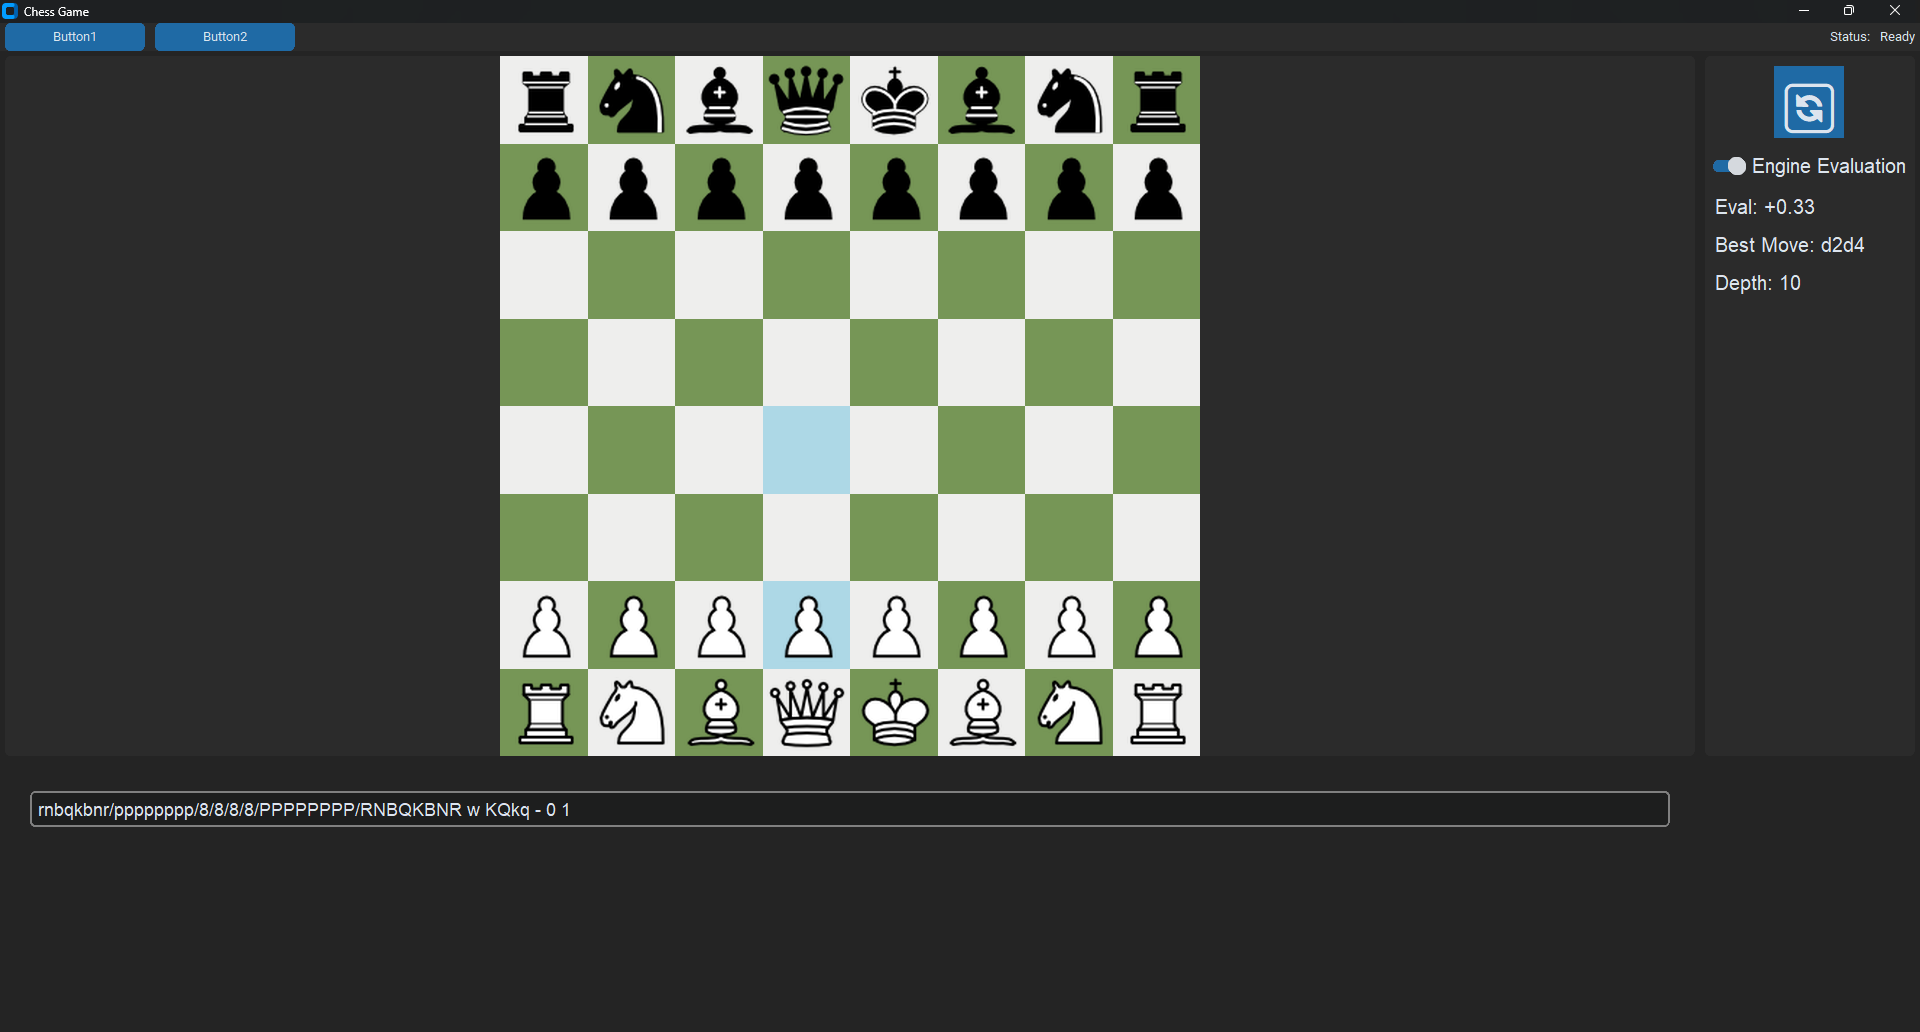
\includegraphics[width=1.0\textwidth]{Imagenes/gui.png}
    \caption{AlphaDeepChess GUI}\label{fig:gui}
\end{figure}

\noindent In~\cref{fig:gui}, the engine evaluation is enabled and displays the current evaluation value, the best move found, and the calculated search depth. In this way, we also ensure a more user-friendly experience.

\vspace{1em}

\noindent In the following chapters, we will present more extensive and detailed information on building the engine.
